%\documentclass[12pt]{article}

\questionheader{ex:s1.3}

%%%%%%%%%%%%%%%%%%
\subsection*{\Conceptual}
%%%%%%%%%%%%%%%%%%
%%%%%%%%%%%%%%%%%%%
\Instructions{There are a lot of constants in this chapter that might be new to you. They can take a little getting used to. Questions \ref{prob_s1.3:constantsa}-\ref{prob_s1.3:constantsb} provide practice working with and interpreting these constants and their relations to each other.}
\begin{question}\label{prob_s1.3:constantsa}
Sketch the curve $\vr(t)=(3\sin t,3\cos t)$. At the point $(0,3)$, label $\hT$ and $\hN$. Give the values of $\kappa$ and $\rho$ at this point as well.
\end{question}
\begin{hint}
The curve is a circle, so you don't need to do any calculus.
\end{hint}
\begin{answer} 
\begin{tikzpicture}
\YEaxis{2}{2}
\YExcoord{.5}{1}
\draw node[shape=circle, minimum size=3cm, draw]{};
\draw (0,1.5) node[vertex]{};
\draw[ultra thick, red, ->] (0,1.5)--(.5,1.5) node[right]{$\hT$};
\draw[ultra thick, blue, ->] (0,1.5)--(0,1) node[below left]{$\hN$};
\end{tikzpicture}
\\
$\rho=3$, $\ka=\frac13$
\end{answer}
\begin{solution}
The curve is a circle of radius 3, centred at the origin. So, the ``circle of best fit" is just the curve itself. $\hT$ is the unit vector tangent to the circle in direction of increasing $t$, and $\hN$ is the unit vector pointing towards the origin.
\begin{center}
\begin{tikzpicture}
\YEaxis{2}{2}
\YExcoord{.5}{1}
\draw node[shape=circle, minimum size=3cm, draw]{};
\draw (0,1.5) node[vertex]{};
\draw[ultra thick, red, ->] (0,1.5)--(.5,1.5) node[right]{$\hT$};
\draw[ultra thick, blue, ->] (0,1.5)--(0,1) node[below left]{$\hN$};
\end{tikzpicture}
\end{center}
The radius of the (osculating) circle is 3, so $\rho=3$ and $\ka=\frac1\rho=\frac13$.
\end{solution}
%%%%%%%%%%%%%%%%%%%
\begin{question}
Consider the circle $\vr(t)=(3\sin t,3\cos t)$. Find $\hT(t)$ and $\hT(s)$. Then, use parts (\eref{CLP317}{thm:curvatureFormulae:part:b}) and (\eref{CLP317}{thm:curvatureFormulae:part:c}) of Theorem~\eref{CLP317}{thm:curvatureFormulae} to find $\hN(t)$ and $\hN(s)$.
\end{question}
\begin{hint}
Because $\vr$ is a circle, you can parametrize it with respect to arclength without using an integral. You found $\ka$ in  Question~\ref{prob_s1.3:constantsa}.
\end{hint}
\begin{answer}
$\hT(t)=(\cos t, -\sin t) $, $\hT(s)=(\cos(s/3),-\sin(s/3))$,\\
$\hN(t)=(-\sin t ,-\cos t)$, $\hN(s)=\left(-\sin(s/3),-\cos(s/3) \right)$
\end{answer}
\begin{solution}
The arclength of $\vr(t)$ traced out by an interval of $t$ of length $\theta$ is $3\theta$. That is, $s=3t$. Our reparametrization of the circle in terms of arclength is $\vR(s)=(3\sin(s/3),3\cos(s/3))$.

We can calculate the vectors tangent to the circle, then normalize them (i.e. make them length one) to find $\hT$.
\begin{align*}
\vv(t)&=\vr'(t)=(3\cos t, -3\sin t) & \hT(s)&=\vR'(s)=(\cos(s/3),-\sin(s/3))\\
\hT(t)&=\frac{\vr'(t)}{|\vr'(t)|}=\frac{(3\cos t, -3\sin t)}{3}=(\cos t, -\sin t) 
\end{align*}
Note $\vR'(s)$, because it's parametrized in terms of arclength, has derivative vectors of length one. So, we don't need to normalize them (although if we did, it wouldn't change anything).

Note also that we can check out answers using Question~\ref{prob_s1.3:constantsa}. In that question, we found $\hT$ was $\hi$ when $t=s=0$; this fits with the vectors we just found.

As in Question~\ref{prob_s1.3:constantsa}, $\ka=\frac13$. So, using Theorem~\eref{CLP317}{thm:curvatureFormulae} Part (\eref{CLP317}{thm:curvatureFormulae:part:b}):
\begin{align*}
\diff{\hT}{s}(s) &= \ka(s)\,\hN(s)\\
\left(-\frac13\sin(s/3)~,~-\frac13\cos(s/3) \right)&=\frac13\hN(s)\\
\left(-\sin(s/3)~,~-\cos(s/3) \right)&=\hN(s)
\end{align*}

Remember $s=3t$. Using Theorem~\eref{CLP317}{thm:curvatureFormulae} Part (\eref{CLP317}{thm:curvatureFormulae:part:c}):
\begin{align*}
\diff{\hT}{t} &= \ka \diff{s}{t} \hN(t)\\
(-\sin t ,-\cos t) &= \frac13 (3) \hN(t)\\
(-\sin t ,-\cos t) &= \hN(t)
\end{align*}
\end{solution}
%%%%%%%%%%%%%%%%%%%
%%%%%%%%%%%%%%%%%%%
\begin{question}
The functon $\vr(t)=(t\cos t, t\sin t)$, $t \ge 0$, defines a spiral centred at the origin. 
Using only geometric intuition (no calculation), predict $\displaystyle\lim_{t \to \infty}\kappa(t)$.
\end{question}
\begin{hint}
When $t$ is large, does the spiral locally look like a circle of large radius, or small?
\end{hint}
\begin{answer}
$\lim\limits_{t \to \infty}\ka(t)=0$
\end{answer}
\begin{solution}
As $t$ increases, the arms of the spiral ``flatten out," looking like a circle of bigger and bigger radius. So, we would expect the curvature to decrease: $\lim\limits_{t \to \infty}\ka(t)=0$. 
\begin{center}
	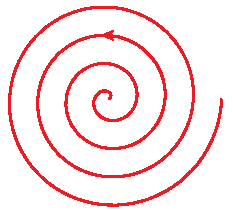
\includegraphics{fig/spiral2d.pdf}
\end{center}
\end{solution}
%%%%%%%%%%%%%%%%%%%
\begin{question}
Let $\vr(t)=(e^t,3t,\sin t)$. What is $\diff{s}{t}$?
\end{question}
\begin{hint}
$\diff{s}{t}=\left| \vv(t)\right|=\left| \vr'(t)\right|$
\end{hint}
\begin{answer}
$\diff{s}{t}=\sqrt{e^{2t}+9+\cos^2 t}$
\end{answer}
\begin{solution}
$\diff{s}{t}=\left| \vv(t)\right|=\left| \vr'(t)\right|=\left| (e^t,3,\cos t)\right|=\sqrt{e^{2t}+9+\cos^2 t}$
\end{solution}
%%%%%%%%%%%%%%%%%%%
\begin{question}\label{prob_s1.3:constantsb}
In Question~\ref{prob_s1.2:spiral} of Section~\eref{CLP317}{sec:reparam},%%%section 1.2
we found that the spiral \[\vr(t) = e^t (\cos t, \sin t)\] parametrized in terms of arclength is 
\[\vR(s)=\frac{s}{\sqrt{2}}\left(\cos\Big(\ln\Big(\frac{s}{\sqrt{2}}\Big)\Big)\,,\,
                 \sin\Big(\ln\Big(\frac{s}{\sqrt{2}}\Big)\Big)\right).\]
                 
Find $\diff{\hT}{s}$ and $\diff{\hT}{t}$ for this curve.
\end{question}
\begin{hint}
$\hT=\frac{\vv(t)}{|\vv(t)|}=\frac{\vr'(t)}{|\vr'(t)|}$
\end{hint}
\begin{answer}
$ \diff{\hT}{t}=\frac1{\sqrt2}\big(-\sin t - \cos t~,~-\sin t + \cos t\big)$\\
$\diff{\hT}{s}=\frac{1}{\sqrt{2}\,s}\left( -\sin \left(\ln\left( s/\sqrt{2}\right)\right)-\cos\left(\ln\left( s/\sqrt{2}\right)\right))~,~-\sin \left(\ln\left( s/\sqrt{2}\right)\right)+\cos \left(\ln\left( s/\sqrt{2}\right)\right)\right)$
\end{answer}
\begin{solution}
\begin{align*}
\hT(t)&=\frac{\vv(t)}{|\vv(t)|}=\frac{\vr'(t)}{|\vr'(t)|}
\intertext{We use the chain rule to differentiate $\vr(t)$.}
&=\frac{\big(e^t(\cos t - \sin t)~,~e^t(\cos t + \sin t)\big)}{\sqrt{e^{2t}(\cos t - \sin t)^2+e^{2t}(\cos t + \sin t)^2}}\\
&=\frac1{\sqrt2}\big(\cos t - \sin t~,~\cos t + \sin t\big)\\
\diff{\hT}{t}&=\frac1{\sqrt2}\big(-\sin t - \cos t~,~-\sin t + \cos t\big)
\intertext{Since $\vR(s)$ is parametrized with respect to arclength, $|\vR'(s)|=1$.}
\hT(s)&=\vR'(s)
\intertext{Making ample use of the chain rule, and setting $U(s)=\left(\ln\left( s/\sqrt{2}\right)\right)$, we have $U'(s)=\frac{1}{s}$:}
\hT(s)&=\frac{1}{\sqrt2}\left( \cos U(s)-\sin U(s)~,~ \cos U(s) + \sin U(s)\right)\\
\diff{\hT}{s}&=\frac{1}{\sqrt{2}\,s}\left( -\sin U(s)-\cos U(s)~,~-\sin U(s)+\cos U(s)\right)
\end{align*}
\end{solution}

%%%%%%%%%%%%%%%%%%%
\begin{question}
In this exercise, we make more precise the sense in which the osculating 
circle is the circle which best approximates a plane curve at a point.
\begin{itemize}\itemsep1pt \parskip0pt \parsep0pt %\itemindent-15pt
\item
By translating and rotating our coordinate system, we
can always arrange that the point is $(0,0)$ and that the curve is
$y=f(x)$ with $f'(0)=0$ and $f''(0)>0$. (We are assuming that
the curvature at the point is nonzero.) 
\item
Let $y=g(x)$ be the bottom half of the circle of radius $r$ which 
is centred at $(0,r)$. 
\end{itemize}
Show that if $f(x)$ and $g(x)$ have the 
same second order Taylor approximation at $x=0$, then $r$ is the 
radius of curvature of $y=f(x)$ at $x=0$.
\end{question}

%\begin{hint}
%\end{hint}

\begin{answer}
See the solution.
\end{answer}

\begin{solution}
The circle  of radius $r$ centred at $(0,r)$ is $x^2+(y-r)^2 = r^2$.
The bottom half of this circle is 
\begin{equation*}
y = g(x) = r - \sqrt{r^2-x^2}
\end{equation*}
So
\begin{alignat*}{3}
g'(x) &=\frac{x}{\sqrt{r^2-x^2}} &
g'(0) &=0 \\
g''(x)&=\frac{1}{\sqrt{r^2-x^2}} +\frac{x^2}{[{r^2-x^2]}^{3/2}}\qquad &
g''(0)&=\frac{1}{r}
\end{alignat*}
As $f(x)$ and $g(x)$ have the same second order Taylor approximation at $x=0$,
$f''(0) = g''(0) = \frac{1}{r}$. 

We may parametrize the curve by $\vr(x) = x\,\hi + f(x)\,\hj$.
So
\begin{alignat*}{3}
\vr'(x)& = \hi +f'(x)\,\hj\qquad &
\vr'(0)& = \hi +f'(0)\,\hj = \hi \\
\vr''(x)& = f''(x)\,\hj &
\vr''(0)& = f''(0)\,\hj \\[0.05in]
\ka(0)& = \frac{|\vr'(0)\times\vr''(0)|}{|\vr'(0)|^3}
 = \frac{|f''(0)\,\hi\times\hj|}{|\hi|^3}
=f''(0)\hidewidth
\end{alignat*}
So $\ka(0)=f''(0)=\frac{1}{r}$ and $r$ is indeed the radius of curvature
of $y=f(x)$ at $x=0$.
\end{solution}


%%%%%%%%%%%%%%%%%%
\subsection*{\Procedural}
%%%%%%%%%%%%%%%%%%
\begin{question}
Given a curve $\vr(t)=(e^t,t^2+t)$, compute the following quantities:
\begin{enumerate}[A.]
\item $\vv(t)$
\item $\va(t)$
\item $\diff{s}{t}$
\item $\hT(t)$
\item $\ka(t)$
\end{enumerate}
\end{question}
\begin{hint}
You can find the last two quantities by making use of the first three. Looking ahead, the formula list in Section~\eref{CLP317}{sec:CurveCompendium} might come in handy. 
\end{hint}
\begin{answer}
\begin{enumerate}[A.]
\item $\vv(t)=(e^t,2t+1)$
\item $\va(t)=(e^t,2)$
\item $\diff{s}{t}=\sqrt{e^{2t}+(2t+1)^2}$
\item $\displaystyle\hT(t)=\left(
 \frac{e^t}{\sqrt{e^{2t}+(2t+1)^2}},
 \frac{2t+1}{\sqrt{e^{2t}+(2t+1)^2}}
 \right)
$
\item $\displaystyle\ka(t)=\dfrac{e^t|1-2t|}{(e^{2t}+(2t+1)^2)^{3/2}}$
\end{enumerate}

\end{answer}
\begin{solution}
\begin{enumerate}[A.]
\item $\vv(t)=\vr'(t)=(e^t,2t+1)$
\item $\va(t)=\vr''(t)=(e^t,2)$
\item $\diff{s}{t}=|\vv(t)|=\sqrt{e^{2t}+(2t+1)^2}$
\item $\displaystyle\hT(t)=\frac{\vv(t)}{|\vv(t)|}=\frac{(e^t,2t+1)}{\sqrt{e^{2t}+(2t+1)^2}}=\left(
 \frac{e^t}{\sqrt{e^{2t}+(2t+1)^2}},
 \frac{2t+1}{\sqrt{e^{2t}+(2t+1)^2}}
 \right)
$
\item $\displaystyle\ka(t)=\frac{|\vv(t) \times \va(t)|}{\left(\diff{s}{t}\right)^3}=\frac{\left| (e^t,2t+1)\times(e^t,2)\right|}{\sqrt{e^{2t}+(2t+1)^2}^3}=\dfrac{e^t|1-2t|}{(e^{2t}+(2t+1)^2)^{3/2}}$
\end{enumerate}

\end{solution}
%%%%%%%%%%%%%%%%%%

%%%%%%%%%%%%%%%%%%%%%%%%%%%
\begin{question}
Find the curvature $\ka(t)$ of $\vr(t)=(\cos t+\sin t , \sin t - \cos t)$.
\end{question}
\begin{hint}
We can calculate $\ka = \dfrac{|\vv(t) \times \va(t)|}{\left| \left(\diff{s}{t}\right)^3\right|}$. We can also figure out what kind of a shape our curve is.
\end{hint}
\begin{answer}
$\ka(t)=\frac{1}{\sqrt{2}}$
\end{answer}
\begin{solution}
\begin{description}
\item[Solution 1:] Note that $(\cos t+\sin t )^2+(\sin t - \cos t)^2=2$ for all $t$. So, the points $(x,y)$ of our curve lie on $x^2+y^2=2$, which is a circle of radius $\sqrt{2}$. Indeed
\begin{align*}
x(t)&= \cos t+\sin t 
=\sqrt{2}\big[\cos t \cos\tfrac{\pi}{4} +\sin t \sin\tfrac{\pi}{4}\big]
\\
&=\sqrt{2}\cos\big(t-\tfrac{\pi}{4}\big)
\\
y(t)&= \sin t-\cos t 
=\sqrt{2}\big[\sin t \cos\tfrac{\pi}{4}-\cos t\sin \tfrac{\pi}{4}\big]
\\
&=\sqrt{2}\sin\big(t-\tfrac{\pi}{4}\big)
\end{align*}
So, $\vr(t)$ circumnavigates a circle of radius $\sqrt{2}$ and consequently has curvature $\ka=\frac{1}{\sqrt{2}}$.
\item[Solution 2:]
We use the formula $\ka = \dfrac{|\vv(t) \times \va(t)|}{\left| \left(\diff{s}{t}\right)^3\right|}$, remembering that $\vv(t)=\vr'(t)$, $\va(t)=\vr''(t)$, and $\diff{s}{t}=\left| \vr'(t)\right|$.
\begin{align*}
\vv(t)&=\vr'(t)=(-\sin t +\cos t, \cos t + \sin t)\\
\va(t)&=\vr''(t)=(-\cos t  -\sin t, -\sin t + \cos t)\\
\vv(t) \times \va(t)&=\big[(-\sin t + \cos t)^2+(\cos t + \sin t)^2\big]\hk=2\hk\\
\diff{s}{t}&=\left|\diff{\vv}{t} \right|=\sqrt{(-\sin t + \cos t)^2+(\cos t + \sin t )^2}=\sqrt2\\
\ka&=\left|\frac{\vv(t) \times \va(t)}{\left(\diff{s}{t}\right)^3}\right|=\left|\frac{2\hk}{\sqrt{2}^3}\right|=\frac{1}{\sqrt 2}
\end{align*}
\end{description}
\end{solution}

%%%%%%%%%%%%%%%%%%%%%%%%%%%
\begin{question}
 Find the minimum and maximum values for the curvature of
the ellipse $x(t)= a \cos t$, $y(t)=b\sin t$. Here $a>b>0$.
\end{question}

\begin{hint} 
The maximum and minimum values of $\ka(t)$ should be
obvious from your formula for $\ka(t)$.
\end{hint}

\begin{answer} 
$\ka_{\rm max}=\frac{a}{b^2}$, $\ka_{\rm min}=\frac{b}{a^2}$.
\end{answer}

\begin{solution} 
 For the given ellipse
\begin{align*}
\vr(t)&= a\cos t\ \hi +b\sin t\ \hj \\
\vv(t)&= -a\sin t\ \hi +b\cos t\ \hj \\
|\vv(t)|& = \sqrt{a^2\sin^2t+b^2\cos^2 t}\\
\va(t)&= -a\cos t\ \hi -b\sin t\ \hj \\
\vv(t)\times\va(t) &=\det\left[\begin{matrix} \hi & \hj & \hk \\
                                        -a\sin t & b\cos t & 0 \\
                                        -a\cos t & -b\sin t & 0 
                                    \end{matrix}\right]
= ab\,\hk\\
\ka(t)&=\frac{|\vv(t)\times\va(t)|}{|\vv(t)|^3}
=\frac{ab}{{[a^2\sin^2t+b^2\cos^2 t]}^{3/2}}
\end{align*}
Hence the maximum (minimum) curvature is achieved when the denominator
is a minimum (maximum) which is the case when $\sin t =0$ ($\cos t=0$).
So $\ka_{\rm max}=\frac{a}{b^2}$ and $\ka_{\rm min}=\frac{b}{a^2}$.
\end{solution}




%%%%%%%%%%%%%%%%%%%%%%%%%%%
\begin{question}[M317 2018A] %1
\begin{enumerate}[(a)]
\item 
Find the curvature of $y=e^x$ at $(0,1)$.
\item
Find the equation of the circle best fitting $y=e^x$
at $(0,1)$.
\end{enumerate}
\end{question}

%\begin{hint} 
%\end{hint}

\begin{answer} 
(a) $\ka(0)=2^{-3/2}$ \qquad
(b) $(x+2)^2+(y-3)^2=8$
\end{answer}

\begin{solution} 
Parametrize the curve by $\vr(t) = t\,\hi +e^t\,\hj$. Then
\begin{align*}
\vv(t) & = \hi + e^t\,\hj  &
\vv(0) & = \hi +\hj &
\frac{ds}{dt} &=|\vv(t)|=\sqrt{1+e^{2t}} &
\hT(t) & = \frac{\vv(t)}{|\vv(t)|} = \frac{\hi+e^t\hj}{\sqrt{1+e^{2t}}}\\
\va(t) & =  e^t\,\hj  &
\va(0) & = \hj \ &
\frac{ds}{dt}(0) &=\sqrt{2} &
\hT(0) & = \frac{\vv(0)}{|\vv(0)|} = \frac{\hi+\hj}{\sqrt{2}}
\end{align*}

(a) We're given $y$ in terms of $x$, so let's use
 Part (\eref{CLP317}{thm:curvatureFormulae:part:e}) of Theorem~\eref{CLP317}{thm:curvatureFormulae}:
 \begin{align*}
 \ka 
&=\frac{\big|\difftwo{y}{x}\big|}
{ {\big[1+\big(\diff{y}{x}\big)^2\big]}^{3/2} } = 
\frac{e^x}
{ {\big[1+\big(e^x\big)^2\big]}^{3/2} } \\
\ka(0)&=\frac{1}{[1+1]^{3/2}}=2^{-3/2}
 \end{align*}


%Since
%\begin{align*}
%\vv(0)\times\va(0) = \hk = \ka(0)\,\big(\frac{ds}{dt}(0)\big)^3\,\hat\vB
%=\ka(0)\,2^{3/2}\, \hat\vB
%\end{align*}
%we have $\ka(0)=2^{-3/2}$ and $\hat\vB=\hk$.
%%%these solutions used \vB, which appears in the NEXT chapter of the text; I've changed it to align more with section 1.3


(b)
\begin{itemize}
\item  The radius of the circle we want is $\rho=\frac{1}{\ka}=2^{3/2}$. If its centre is at $(a,b)$, then the circle will have equation $(x-a)^2+(y-b)^2=2^3$. So, we will find its centre.

\item The unit vector $\hN$ points from our point $(0,1)$ towards the centre of the circle. Since the radius of the circle is $2^{3/2}$, the centre of the circle will be at $(0,1)+2^{3/2}\hN$. So, we'll find $\hN$.

\item Since $\hN$ is a unit vector perpendicular to $\hT=\dfrac{\hi+\hj}{\sqrt 2}$, we know $\hN$ will be either $\dfrac{\hi-\hj}{\sqrt 2}$ or $\dfrac{-\hi+\hj}{\sqrt 2}$.

\item Using Part~(\eref{CLP317}{clpcurvesthm:curvatureFormulae:partd}) of the proof of Theorem~\eref{CLP317}{thm:curvatureFormulae}:
\begin{align*}
\vv(t) \times \va(t) &= \ka\left(\diff{s}{t}\right)^3\hT \times \hN\\
(\hi+\hj)\times(\hj)&=2^{-3/2}\left(\sqrt2 \right)^3\frac{\hi+\hj}{\sqrt 2}\times\hN\\
\hk &=\frac{1}{\sqrt2}(\hi + \hj)\times\hN\\
\hN&=\frac{-\hi+\hj}{\sqrt2}
 \end{align*}
So, the centre of our circle is at point $(0,1)+\rho\hN=(0,1)+2^{3/2}\frac{-\hi+\hj}{2^{1/2}}=(-2,3)$. Then the equation of the circle is $(x+2)^2+(y-3)^2=8$.
\end{itemize}
%We have
%\begin{equation*}
%\hN(0) = \hat\vB(0)\times\hT(0) = \frac{1}{\sqrt{2}}\hk\times(\hi+\hj)
%=\frac{1}{\sqrt{2}}(-\hi+\hj)
%\end{equation*}
%so that the radius of curvature is $\frac{1}{\ka(0)}=2^{3/2}$ and 
%centre of curvature is
%\begin{align*}
%(0,1) + \frac{1}{\ka(0)}\hN(0) = (0,1) +2^{3/2} 2^{-1/2}(-1,1)=(-2,3)
%\end{align*}
%and the equation of the osculating circle is 
%$(x+2)^2+(y-3)^2=8$. 
\end{solution}


%%%%%%%%%%%%%%%%%%%%%%%%%%%%%%%
\begin{question}[M317 2011A] %1
\item   %1
Consider the motion of a thumbtack stuck in the tread of a tire which 
is on a bicycle moving at constant speed. This motion is given by 
the parametrized curve 
\begin{equation*}
\vr(t) = \big(t - \sin t\,,\, 1 - \cos t\big)
\end{equation*}
with $t > 0$.
\begin{enumerate}[(a)]
\item
Sketch the curve in the $xy$-plane for $0 < t < 4\pi$.
\item
Find and simplify the formula for the curvature $\kappa(t)$.
\item
Find the radius of curvature of the osculating circle to 
$\vr(t)$ at $t = \pi$.
\item
Find the equation of the osculating circle to $\vr(t)$ at $t = \pi$.
\end{enumerate}
\end{question}

\begin{hint} 
For part (a), determine $\vr(0)$, $\vr(\pi)$, $\vr(2\pi)$, $\vr(3\pi)$, and $\vr(4\pi)$, to help you map out the motion. Also visualize the thumbtack as the wheel moves.

For part (d), use the fact that you only care about $t=\pi$: where is this on your sketch? What does that mean about the direction of $\hN$?
\end{hint}

\begin{answer} 
(a)
\begin{center}
    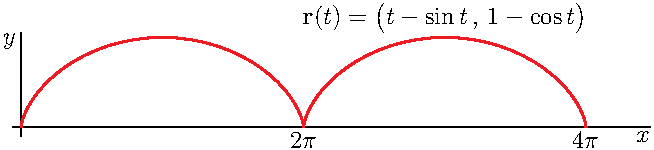
\includegraphics{fig/tack.pdf}
\end{center}

(b) $\ka(t) = \frac{1}{2^{3/2}\sqrt{1-\cos t}}$\qquad
(c) $4$\qquad
(d) $(x-\pi)^2 +(y+2)^2 = 16$
\end{answer}

\begin{solution} (a)
Think of 
\begin{equation*}
\vr(t) = (t,1) - (\sin t,\cos t)
\end{equation*}
The $(t,1)$ part gives the position of the centre of the wheel at time
$t$. The other part gives the position of the thumbtack with respect to
the centre of the wheel. In particular,
\begin{itemize}\itemsep1pt \parskip0pt \parsep0pt %\itemindent-15pt
\item[$\circ$]
at time $t=0$, $\vr(0) = (0,0)$. The thumbtack is on the ground (i.e. at $y=0$).
\item[$\circ$]
At time $t=\pi$, $\vr(\pi) = (\pi,2)$. The thumbtack is at its highest point (i.e. at $y=2$) and is above the centre of the wheel at $x=\pi$.
\item[$\circ$]
At time $t=2\pi$, $\vr(2\pi) = (2\pi,0)$. The thumbtack is back on the ground (i.e. at $y=0$) and is below the centre of the wheel at $x=2\pi$.
\item[$\circ$]
At time $t=3\pi$, $\vr(3\pi) = (3\pi,2)$. The thumbtack is again at its highest point (i.e. at $y=2$) and is above the centre of the wheel at $x=3\pi$.
\item[$\circ$]
At time $t=4\pi$, $\vr(4\pi) = (4\pi,0)$. The thumbtack is back on the ground (i.e. at $y=0$) and is below the centre of the wheel at $x=4\pi$.
\end{itemize}
Here is a sketch of the curve.
\begin{center}
    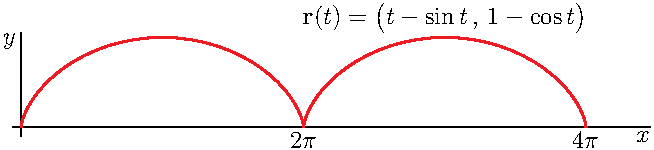
\includegraphics{fig/tack.pdf}
\end{center}

(b) Since 
\begin{align*}
\vr(t) &= \big(t - \sin t\,,\, 1 - \cos t\big) \\
\vv(t) =\vr'(t)&= \big(1-\cos t\,,\, \sin t\big) \\
\diff{s}{t}(t)=|\vv(t)|&=\sqrt{2-2\cos t} \\
\va(t) = \vv'(t)&=\big(\sin t\,,\, \cos t\big)  \displaybreak[0]\\
\vv(t)\times \va(t)&=\det\left[\begin{matrix}\hi&\hj&\hk\\[0.03in] 
     1-\cos t & \sin t & 0 \\
     \sin t  & \cos t & 0\end{matrix}\right]
=\big(\cos t-1\big)\,\hk
\end{align*}
the curvature
\begin{align*}
\ka(t) =\frac{|\vv(t)\times\va(t)|}{|\vv(t)|^3}
       =\frac{|\cos t-1|}{(2-2\cos t)^{3/2}}
       =\frac{1}{2^{3/2}\sqrt{1-\cos t}}
\end{align*}

(c) The radius of curvature at time $t=\pi$ is
\begin{equation*}
\rho(\pi) = \frac{1}{\ka(\pi)}
          = \frac{1}{1/2^{3/2}\sqrt{2}}
          =4
\end{equation*}

(d) At time $\pi$, the tack is at $\vr(\pi)=(\pi,2)$, which is at the top 
of its trajectory. Looking at the sketch in part (a), we see that,
at that time $\hN(\pi) = -\hj$.
So the osculating circle at time $t=\pi$ has center
\begin{equation*}
\vr(\pi) + \rho(\pi) \hN(\pi)
=(\pi,2) + 4(0,-1)
=(\pi,-2)
\end{equation*}
and radius $\rho(\pi)=4$. So the equation  of the osculating circle
at time $\pi$ is
\begin{equation*}
(x-\pi)^2 +(y+2)^2 = 16
\end{equation*}
\end{solution}





%%%%%%%%%%%%%%%%%%
\subsection*{\Application}
%%%%%%%%%%%%%%%%%%

%%%%%%%%%%%%%%%%%%%%%%%%%%%
\begin{question}
 Find the curvature $\ka$ as a function of arclength $s$ 
(measured from $(0,0)$) for the curve
\begin{equation*}
x(\theta)=\int_0^\theta \cos\big(\half\pi t^2\big)dt\quad \quad
y(\theta)=\int_0^\theta \sin\big(\half\pi t^2\big)dt
\end{equation*}
\end{question}

\begin{hint} 
You should find that $s=\theta$!
\end{hint}

\begin{answer} 
$\ka(s)=\pi s$
\end{answer}

\begin{solution} 
The velocity vector is
\begin{equation*}
\vv(\theta)=x'(\theta)\,\hi+y'(\theta)\,\hj
= \cos\big(\half\pi\theta^2\big)\,\hi + \sin\big(\half\pi\theta^2\big)\,\hj
\end{equation*}
Consequently the speed
\begin{equation*}
\diff{s}{\theta}(\theta)= |\vv(\theta)|=1
\implies s(\theta)=\theta+s(0)
\end{equation*}
Since $s(\theta)$ is zero when $\theta=0$, we have $s(\theta)=\theta$ and hence
\begin{equation*}
\hT(s)=\vv(s)
= \cos\big(\half\pi s^2\big)\,\hi + \sin\big(\half\pi s^2\big)\,\hj
\end{equation*}
so that
\begin{equation*}
\ka(s)=\left|\diff{\hT}{s}(s)\right|
=\big|-\pi s\sin\big(\half\pi s^2\big)\,\hi
+\pi s \cos\big(\half\pi s^2\big)\,\hj\big|
=\pi s
\end{equation*}
\end{solution}


%%%%%%%%%%%%%%%%%%%%%%%%%%%
\begin{question}[M317 2011D]  %3
Let $C$ be the curve in $\bbbr^2$ given by the graph of the function
$y=\frac{x^3}{3}$. Let $\kappa(x)$ be the curvature of $C$ at the point 
$(x, x^3/3)$. Find all points where $\ka(x)$ attains its maximal values,
or else explain why such points do not exist. What are the limits of 
$\kappa(x)$ as $x \rightarrow \infty$ and
$x \rightarrow -\infty$?
\end{question}

\begin{hint} 
Since $\ka(x)$ is never negative, $\ka(x)$ is maximum when $\ka^2(x)$ is maximum. The latter is easier to compute.
\end{hint}

\begin{answer} 
The maximum values occur at $(x,y)=\pm \big(1/\root{4}\of{5}\,,\,
                 \frac{1}{3}5^{-3/4}\big)$.

The limits $\lim_{x\rightarrow\pm\infty}\ka(x) = 0$.
\end{answer}

\begin{solution} 
The curve is $y=y(x)=\nicefrac{x^3}{3}$. Since $y'(x) = x^2$ and
$y''(x) = 2x$, the curvature is
\begin{align*}
\ka(x)
&=\frac{\big|\difftwo{y}{x}(x)\big|}
  {\Big[1+\big(\diff{y}{x}(x)\big)^2\Big]^{3/2}}
=\frac{\big|2x\big|}
  {\big[1+x^4\big]^{3/2}}
\end{align*}
 We'd like to find the critical points of $\ka(x)$, but differentiating it looks messy. Since $\ka(x)$ has only nonnegative values, its maxima correspond the the maxima of the function $\ka^2(x)$. So, we find the critical points of $\ka^2(x)$ instead, to save ourselves some computational toil.
\begin{align*}
0&=\diff{\hfill}{x}\ka(x)^2
=\diff{\hfill}{x}\frac{4x^2}{{(1+x^4)}^3}
=\frac{8x}{{(1+x^4)}^3} - 3\frac{16x^5}{{(1+x^4)}^4}
=\frac{8x(1+x^4)-3\times 16x^5}{{(1+x^4)}^4} \\
&=\frac{8x(1-5x^4)}{{(1+x^4)}^4}
\end{align*}
Note that $\ka(0)=0$ and $\ka(x)\rightarrow 0$ as $x\rightarrow\pm \infty$.
So the maximum occurs when $x=\pm 1/\root{4}\of{5}$.
\end{solution}

%\begin{question}[M317 2008D] %2
%Find the point in the first quadrant where the graph of the function 
%$y = \frac{1}{3} x^3$ has maximal curvature.
%\end{question}

%\begin{hint} 
%Find a formula for $\kappa(x)$, then maximize it using methods from first-semester calculus.
%\end{hint}

%\begin{answer} 
%$\big(\frac{1}{5^{1/4}}\,,\,\frac{1}{3\cdot 5^{3/4}}\big)$
%\end{answer}

%\begin{solution} 
%The specified curve is the graph of $y=f(x)$ with $f(x)=\frac{1}{3}x^3$.
%So, from \S \eref{CLP317}{sec:CurveCompendium} in the CLP-4 text, 
%the curvature is
%\begin{align*}
%\kappa(x) =\frac{|f''(x)|}{[{1+f'(x)^2]}^{3/2}}
%          =\frac{2|x|}{{[1+x^4]}^{3/2}}
%\end{align*}
%We are interested only in $x\ge 0$, so
%\begin{align*}
%\kappa(x) =\frac{2x}{{[1+x^4]}^{3/2}}
%\end{align*}
%As
%\begin{align*}
%\ka'(x) &= \frac{2}{{[1+x^4]}^{3/2}} 
%             -\frac{3}{2}\frac{2x(4x^3)}{{[1+x^4]}^{5/2}}
%=\frac{2-10x^4}{{[1+x^4]}^{5/2}}
%\end{align*}
%vanishes when $x=1/\root{4}\of{5}$, the only critical point of $\ka(x)$ occurs there. 

%We might want to satisfy ourselves that $x=1/\root{4}\of{5}$
%is a point of \emph{maximum} curvature (as opposed to, say, a point of minimum curvature). A sketch of $y=\frac{1}{3}x^3$ suggests this is the case, but we can also use the second derivative test:
%$
%\ka''(x)=\dfrac{60x^3(-1+x^4)}{(1+x^4)^{7/3}}$, so $\ka''(1/\root{4}\of{5})<0$, and our critical point is indeed the location of the maximum curvature.

%So, the curvature is maximum at the point
%$x=\frac{1}{5^{1/4}}$, $y=\frac{1}{3\cdot 5^{3/4}}$.


%\end{solution}


